\documentclass{article}
\title{Analysis of Linux Schedulers}
\author{Carl Cortright}
\date{December 3, 2016}
\usepackage{listings}
\usepackage{graphicx}
\usepackage[section]{placeins}
\usepackage{float}
\usepackage[margin=1.5in]{geometry}

\begin{document}
\maketitle

\section{Abstract}

In this paper I analyze the performance of three standard Linux schedulers, the FIFO scheduler, the real time scheduler, and the completely fair scheduler. I used three C programs to evaluate each of these schedulers over varying conditions, including during intensive IO and CPU operations. By charting my results to help visualize the performance of each scheduler, I am able to conclude that the standard Linux completely fair scheduler is the best scheduler for most situations.

\section{Introduction}

Operating system schedulers are systems that are unseen, but they play a huge role in every day life, helping run our everyday computers so they don’t appear to freeze, preventing fatal scheduling bugs in our financial systems, even ensuring that life-critical systems on aircraft continue functioning. Different operating schedulers perform differently depending on the operations they are scheduling. I will start by designing an experiment to evaluate three different schedulers, the standard Linux completely fair scheduler, real time scheduler, and the naive first in first out scheduler. Testing the schedulers under varying processor utilizations, priorities of children, and IO vs CPU operations, I ran extensive tests of the performance of each scheduler. I then evaluate these systems on their performance using standard benchmarks, including how much system, user, and real time they take on the processor. Lastly, I compare the systems to each other, analyzing their advantages/disadvantages in any given situation.

\section{Experimental Design}

To properly evaluate the performance of operating schedulers, it is important to have a proper experimental design that minimizes outside factors including other processes that might produce uneven results over time. For standardization purposes, I performed this experiment on a Dell Inspiron 5520 with a 4-core Intel i7 processor, 8GB (DDR3) of memory, and upgraded Samsung SSD (read/write up to 520mb/sec). At the time of the experiment, the machine was also running a Deep-Q learning program that had been running for days. The Deep-Q Learning program was consistently using approximately 500MB of RAM along with 25 percent processor utilization. After multiple runs of the test program, I was able to determine that this program had no noticeable effect on the results of the experiment.

To test the performance of each scheduler, I wrote three different c programs, one to test the schedulers under CPU intensive tasks, one to test the schedulers under IO intensive task, and one to test both at the same time. Each of these C programs had different arguments that could test different configurations; the CPU program was statistically calculating pi and could specify the number of children and iterations of the pi calculator, along with scheduling policy and if priority should be varied between children; the IO program was writing and reading a file and could specify number of processes, policy, if priority should be varied, transfer size, and block size; the mixed program calculated pi before doing read/write operations and it could specify number of children, policy, varied process priority, transfer size, block size, and iterations. Usage for each of the three programs is described below:

\begin{lstlisting}[language=bash]
  $./pi-sched <children> <iterations> <policy>
  <vary priority>
  $./rw-sched <number of processes> <policy>
  <vary priority> <transfer size> <block size>
  $./mixed-sched <number of processes> <policy>
  <vary priority> <transfer size> <block size> <iterations>
\end{lstlisting}

Each of the programs forks the number of processes specified and does the IO or CPU intensive operations. I used the c resource library’s getrusage() command to get relevant user and system time usages for the children processes. Separately I used the time library’s clockgettime() command to get real time data for how long each run took to execute. For the programs that involved reading and writing, it was important that each child process had its own set of input and output files to work with, because if they were all reading and writing to the same file, there would be a clear bottleneck that would skew our experiments results. Before I started the timers, I wrote data from /dev/random to separate input files for each process. It was this process that made using time time utility unpractical for the experiment. The time utility would have included these operations in its calculation, and in order to get accurate results for the experiment it was important to only time the child processes.

To get consistent results for the CPU and IO intensive operations, I picked fixed values for iterations, transfer size, and block size. For the the number of iterations to calculate Pi, I fixed the value at 10 million iterations. For the IO operations, I picked a fixed transfer size of 1KB (1024 Bytes) with an 8 Byte block size.

To get a wide range of results, I wrote a bash script that ran each of the three programs 18 times. This amounted to 54 test cases. For each program, I tested each scheduler over varying priorities and number of child processes. Each scheduler was tested over three cases, when it had 5 children, 50 children, and 500 children, without varying priority. Then, the same tests were repeated, except this time priority was varied. To make it easier to analyze, each of the test programs outputted its configuration along with results in the standard CSV format, making it easy to process the data in a standard Google Sheet.

\section{Results}

When analyzing the results of my experiments, it was important to recognize the metrics that best evaluated the performance of each scheduler. I chose to use “real time” as my main metric of evaluation, along with real time per process, calculated after the experiment. In my analysis, I will look some at the effects CPU or IO has on system and user time, but the focus will be on the real time metrics.

\subsection{CPU Task Results}
To assess the performance of the different schedulers against each other, I took the data collected and graphed it using bar graphs, once with varied priorities, and then again without varied priorities. I used the trial with 500 processes for each so that the distinction would be more clear:

\begin{figure}[H]
  \centering
  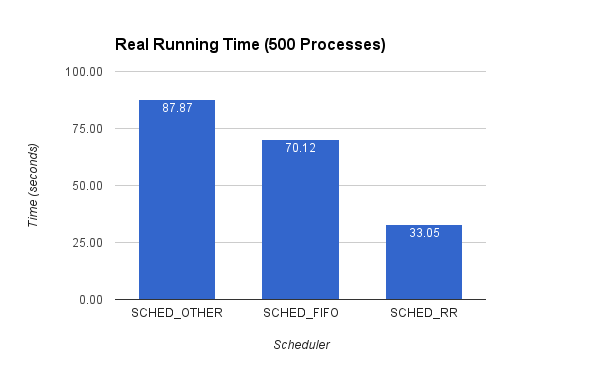
\includegraphics[width=0.8\linewidth]{CPUNotVaried.png}
  \caption{Running times of CPU tasks on different schedulers, 500 child processes without varying priority}
\end{figure}

I then did the same with varied priorities. Notice for later that the completely fair scheduler has a significantly faster running time than the other two which got marginally slower. For reference, it has a time per process of only 0.012 seconds which was the fastest of any of the trials.

\begin{figure}[H]
  \centering
  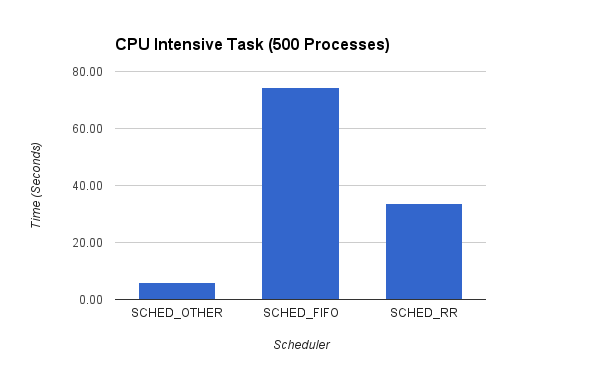
\includegraphics[width=0.8\linewidth]{CPUVaried.png}
  \caption{Running times of CPU tasks on different schedulers, 500 child processes with varied priority}
\end{figure}

 Because the completely fair scheduler had such remarkable performance, I decided to dive a bit deeper and plot a line graph of the Time per Process vs. Number of Processes.

\begin{figure}[H]
  \centering
  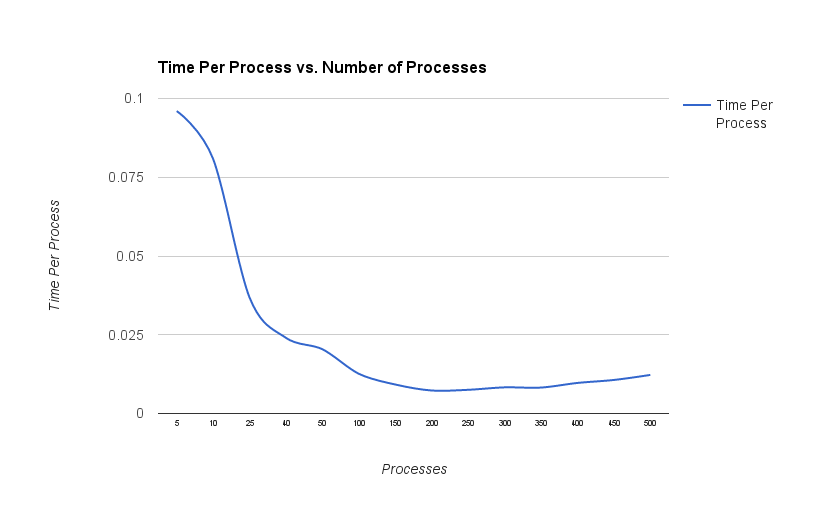
\includegraphics[width=0.8\linewidth]{CPUProcessesGraph.png}
  \caption{Improvement of running time per process over time with the varied completely fair scheduler}
\end{figure}


\subsection{IO Task Results}

To allow for accurate comparisons, I graphed the same trials as the CPU task section. Again, I graphed it using bar graphs, once with varied priorities and once without varied priorities, using 500 processes.


\begin{figure}[H]
  \centering
  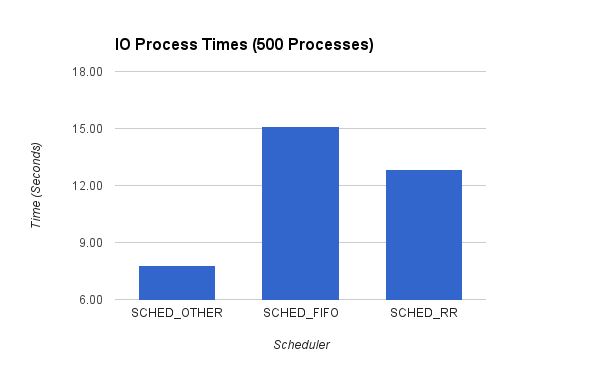
\includegraphics[width=0.8\linewidth]{IONotVaried.png}
  \caption{Running times of IO tasks on different schedulers, 500 child processes without varying priority}
\end{figure}

I then did the same for varied priorities, plotting the running times for the 500 process trials on a bar graph. Notice the continued pattern of the completely fair scheduler maintaining its speed even as the number of processes increases by an order of magnitude.


\begin{figure}[H]
  \centering
  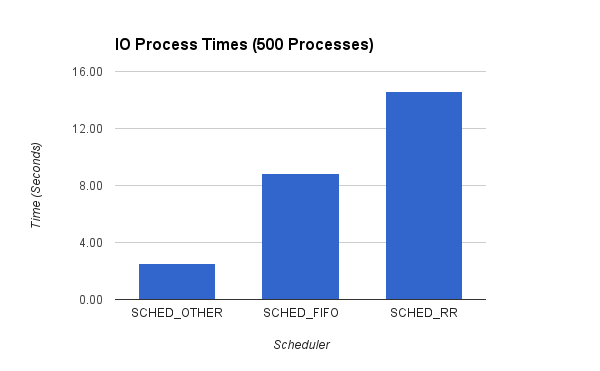
\includegraphics[width=0.8\linewidth]{IOVaried.png}
  \caption{Running times of IO tasks on different schedulers, 500 child processes with varied priority}
\end{figure}

Another thing to notice with the IO processes is that the trials that had fewer processes were dramatically slower per process. I also included this histogram.


\begin{figure}[H]
  \centering
  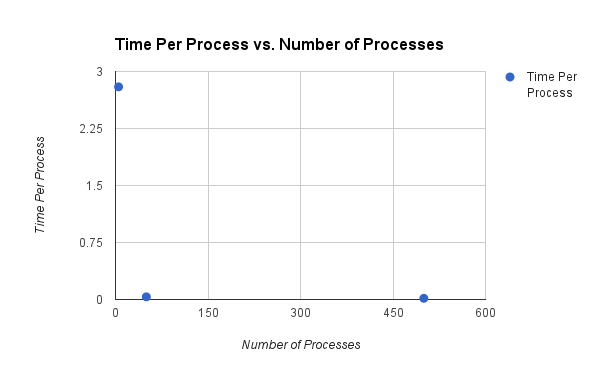
\includegraphics[width=0.8\linewidth]{IOAverageRuntime.png}
  \caption{Average runtime of a process for IO operations}
\end{figure}

\subsection{Mixed Task Results}

I produced the same graphs for the mixed tasks. The results were very similar to what would be expected from adding the IO and CPU tasks together. All of the data for my results section is listed in Appendix A.


\begin{figure}[H]
  \centering
  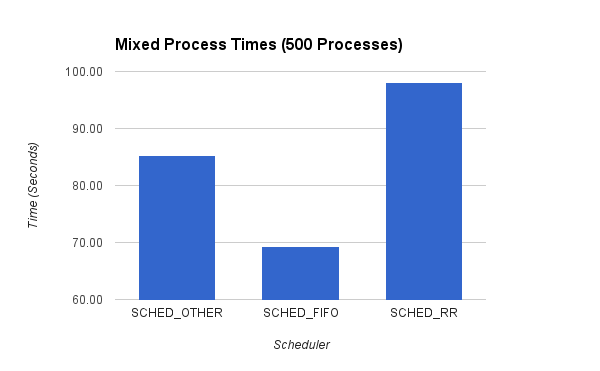
\includegraphics[width=0.8\linewidth]{MixedNotVaried.png}
  \caption{Running times of Mixed tasks on different schedulers, 500 child processes without varied priority}
\end{figure}


\begin{figure}[H]
  \centering
  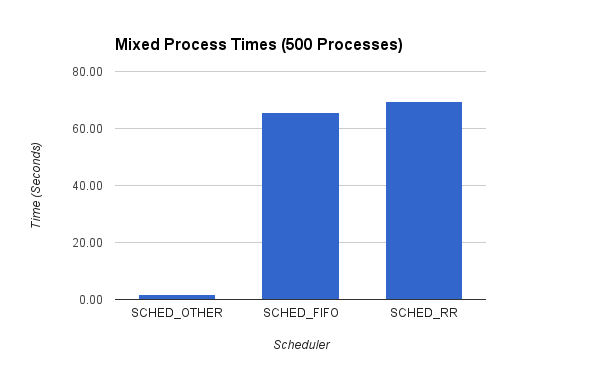
\includegraphics[width=0.8\linewidth]{MixedVaried.png}
  \caption{Running times of Mixed tasks on different schedulers, 500 child processes with varied priority}
\end{figure}

\section{Analysis}

The naive first in first out scheduler was almost always the slowest except when I varied priorities in the trials that involved IO operations, causing the real time scheduler to slow down. This was likely the result of having to initiate and prioritize new IO operations, interrupting the current process. It also makes sense because I started the low priority processes first, meaning they would be more likely to be interrupted.

For all of the trials with memory accesses, the trials with 5 processes had significantly slower time of completion per child process. I’m guessing this was the result of the slowness of memory access. The CPU and DMA unit can coordinate to fetch a lot of the memory at once, but that fetch time is slow, making the trials with a higher number of processes faster per process.

Not mentioned in the results but relevant to our conclusion, was the fact that the IO processes took more system time and the CPU process took more user time. IO processes have to make more systems calls, meaning the machine will spend more time in kernel mode. CPU processes have to spend more time executing code in user mode, driving their user time up.

Throughout all of the trials, a clear trend emerged that the standard Linux kernel completely fair scheduler with varying priority was the best of all the different schedulers. In many cases, it was orders of magnitude faster than the other methods, making it the obvious scheduler of choice for many general applications. The reason it is so fast is most likely due to both its efficacy as a scheduling method as well as the fact that developers likely spent much more time implementing and testing, causing the performance to increase.

\section{Conclusion}

Operating system schedulers play a crucial role in running the computer systems we rely on every day. I have analyzed the performance of three Linux schedulers and determined that the standard Linux completely fair scheduler is optimal for nearly all general purpose tasks such as for standard servers and laptops. That isn’t to say that there aren’t situation where the other schedulers could be useful. For example, the Linux real time scheduler, if being used to control life-critical systems, could be the scheduler of choice.

\section{Appendix A: Data}

\subsection{CPU Intensive Data}

\begin{table}[H]
\centering
\label{my-label}
\resizebox{\columnwidth}{!}{
\begin{tabular}{lllllllll}
Task     & Scheduler    & Number of Processes & Vary Priority & Iterations    & System Time & User Time & Real Time & Real Time Per Process \\
pi-sched & SCHED\_OTHER & 5                   & FALSE         & 10,000,000.00 & 0.00        & 0.52      & 0.52      & 0.104                 \\
pi-sched & SCHED\_OTHER & 50                  & FALSE         & 10,000,000.00 & 0.00        & 0.94      & 5.34      & 0.1068                \\
pi-sched & SCHED\_OTHER & 500                 & FALSE         & 10,000,000.00 & 0.00        & 1.42      & 87.87     & 0.17574               \\
pi-sched & SCHED\_FIFO  & 5                   & FALSE         & 10,000,000.00 & 0.00        & 0.94      & 0.94      & 0.188                 \\
pi-sched & SCHED\_FIFO  & 50                  & FALSE         & 10,000,000.00 & 0.00        & 0.94      & 7.21      & 0.1442                \\
pi-sched & SCHED\_FIFO  & 500                 & FALSE         & 10,000,000.00 & 0.00        & 0.94      & 70.12     & 0.14024               \\
pi-sched & SCHED\_RR    & 5                   & FALSE         & 10,000,000.00 & 0.00        & 0.75      & 0.75      & 0.15                  \\
pi-sched & SCHED\_RR    & 50                  & FALSE         & 10,000,000.00 & 0.00        & 0.98      & 3.33      & 0.0666                \\
pi-sched & SCHED\_RR    & 500                 & FALSE         & 10,000,000.00 & 0.00        & 1.12      & 33.05     & 0.0661                \\
pi-sched & SCHED\_OTHER & 5                   & TRUE          & 10,000,000.00 & 0.00        & 0.74      & 1.62      & 0.324                 \\
pi-sched & SCHED\_OTHER & 50                  & TRUE          & 10,000,000.00 & 0.00        & 0.95      & 2.33      & 0.0466                \\
pi-sched & SCHED\_OTHER & 500                 & TRUE          & 10,000,000.00 & 0.00        & 0.98      & 6.11      & 0.01222               \\
pi-sched & SCHED\_FIFO  & 5                   & TRUE          & 10,000,000.00 & 0.00        & 0.98      & 0.98      & 0.196                 \\
pi-sched & SCHED\_FIFO  & 50                  & TRUE          & 10,000,000.00 & 0.00        & 0.98      & 6.52      & 0.1304                \\
pi-sched & SCHED\_FIFO  & 500                 & TRUE          & 10,000,000.00 & 0.00        & 0.98      & 74.34     & 0.14868               \\
pi-sched & SCHED\_RR    & 5                   & TRUE          & 10,000,000.00 & 0.00        & 1.48      & 1.06      & 0.212                 \\
pi-sched & SCHED\_RR    & 50                  & TRUE          & 10,000,000.00 & 0.00        & 0.98      & 3.54      & 0.0708                \\
pi-sched & SCHED\_RR    & 500                 & TRUE          & 10,000,000.00 & 0.00        & 1.28      & 33.70     & 0.0674
\end{tabular}
}
\end{table}

\subsection{IO Intensive Data}
\begin{table}[H]
\centering
\label{my-label}
\resizebox{\columnwidth}{!}{
\begin{tabular}{llllllllllllllllllllllll}
Task     & Scheduler    & Number of Processes & Vary Priority & Transfer Size & Blocksize & System Time & User Time & Real Time & Time Per Process &  &  &  &  &  &  &  &  &  &  &  &  &  &  \\
rw-sched & SCHED\_OTHER & 5                   & FALSE         & 1,024.00      & 8.00      & 0.00        & 0.00      & 13.99     & 2.798            &  &  &  &  &  &  &  &  &  &  &  &  &  &  \\
rw-sched & SCHED\_OTHER & 50                  & FALSE         & 1,024.00      & 8.00      & 0.00        & 0.00      & 1.75      & 0.035            &  &  &  &  &  &  &  &  &  &  &  &  &  &  \\
rw-sched & SCHED\_OTHER & 500                 & FALSE         & 1,024.00      & 8.00      & 0.12        & 0.00      & 7.78      & 0.01556          &  &  &  &  &  &  &  &  &  &  &  &  &  &  \\
rw-sched & SCHED\_FIFO  & 5                   & FALSE         & 1,024.00      & 8.00      & 0.00        & 0.16      & 10.40     & 2.08             &  &  &  &  &  &  &  &  &  &  &  &  &  &  \\
rw-sched & SCHED\_FIFO  & 50                  & FALSE         & 1,024.00      & 8.00      & 0.40        & 0.00      & 1.79      & 0.0358           &  &  &  &  &  &  &  &  &  &  &  &  &  &  \\
rw-sched & SCHED\_FIFO  & 500                 & FALSE         & 1,024.00      & 8.00      & 0.40        & 0.00      & 15.09     & 0.03018          &  &  &  &  &  &  &  &  &  &  &  &  &  &  \\
rw-sched & SCHED\_RR    & 5                   & FALSE         & 1,024.00      & 8.00      & 0.24        & 0.00      & 0.86      & 0.172            &  &  &  &  &  &  &  &  &  &  &  &  &  &  \\
rw-sched & SCHED\_RR    & 50                  & FALSE         & 1,024.00      & 8.00      & 0.00        & 0.40      & 1.42      & 0.0284           &  &  &  &  &  &  &  &  &  &  &  &  &  &  \\
rw-sched & SCHED\_RR    & 500                 & FALSE         & 1,024.00      & 8.00      & 0.00        & 0.00      & 12.82     & 0.02564          &  &  &  &  &  &  &  &  &  &  &  &  &  &  \\
rw-sched & SCHED\_OTHER & 5                   & TRUE          & 1,024.00      & 8.00      & 0.12        & 0.00      & 0.80      & 0.16             &  &  &  &  &  &  &  &  &  &  &  &  &  &  \\
rw-sched & SCHED\_OTHER & 50                  & TRUE          & 1,024.00      & 8.00      & 0.40        & 0.00      & 1.68      & 0.0336           &  &  &  &  &  &  &  &  &  &  &  &  &  &  \\
rw-sched & SCHED\_OTHER & 500                 & TRUE          & 1,024.00      & 8.00      & 0.00        & 0.80      & 2.51      & 0.00502          &  &  &  &  &  &  &  &  &  &  &  &  &  &  \\
rw-sched & SCHED\_FIFO  & 5                   & TRUE          & 1,024.00      & 8.00      & 0.80        & 0.00      & 11.23     & 2.246            &  &  &  &  &  &  &  &  &  &  &  &  &  &  \\
rw-sched & SCHED\_FIFO  & 50                  & TRUE          & 1,024.00      & 8.00      & 0.00        & 0.40      & 1.85      & 0.037            &  &  &  &  &  &  &  &  &  &  &  &  &  &  \\
rw-sched & SCHED\_FIFO  & 500                 & TRUE          & 1,024.00      & 8.00      & 0.00        & 0.00      & 8.87      & 0.01774          &  &  &  &  &  &  &  &  &  &  &  &  &  &  \\
rw-sched & SCHED\_RR    & 5                   & TRUE          & 1,024.00      & 8.00      & 0.12        & 0.00      & 6.79      & 1.358            &  &  &  &  &  &  &  &  &  &  &  &  &  &  \\
rw-sched & SCHED\_RR    & 50                  & TRUE          & 1,024.00      & 8.00      & 0.40        & 0.00      & 1.60      & 0.032            &  &  &  &  &  &  &  &  &  &  &  &  &  &  \\
rw-sched & SCHED\_RR    & 500                 & TRUE          & 1,024.00      & 8.00      & 0.00        & 0.00      & 14.57     & 0.02914          &  &  &  &  &  &  &  &  &  &  &  &  &  &
\end{tabular}
}
\end{table}

\subsection{Mixed Data}

\begin{table}[H]
\centering
\label{my-label}
\resizebox{\columnwidth}{!}{
\begin{tabular}{llllllllllllllllllllllll}
Task        & Scheduler    & Number of Processes & Vary Priority & Iterations    & Transfer Size (Bytes) & Blocksize (Bytes) & System Time & User Time & Real Time &  &  &  &  &  &  &  &  &  &  &  &  &  &  \\
mixed-sched & SCHED\_OTHER & 5                   & FALSE         & 10,000,000.00 & 1,024.00              & 8.00              & 0.40        & 1.56      & 1.57      &  &  &  &  &  &  &  &  &  &  &  &  &  &  \\
mixed-sched & SCHED\_OTHER & 50                  & FALSE         & 10,000,000.00 & 1,024.00              & 8.00              & 0.00        & 0.86      & 5.52      &  &  &  &  &  &  &  &  &  &  &  &  &  &  \\
mixed-sched & SCHED\_OTHER & 500                 & FALSE         & 10,000,000.00 & 1,024.00              & 8.00              & 0.40        & 1.36      & 85.20     &  &  &  &  &  &  &  &  &  &  &  &  &  &  \\
mixed-sched & SCHED\_FIFO  & 5                   & FALSE         & 10,000,000.00 & 1,024.00              & 8.00              & 0.00        & 0.90      & 3.18      &  &  &  &  &  &  &  &  &  &  &  &  &  &  \\
mixed-sched & SCHED\_FIFO  & 50                  & FALSE         & 10,000,000.00 & 1,024.00              & 8.00              & 0.40        & 0.89      & 9.05      &  &  &  &  &  &  &  &  &  &  &  &  &  &  \\
mixed-sched & SCHED\_FIFO  & 500                 & FALSE         & 10,000,000.00 & 1,024.00              & 8.00              & 0.00        & 0.90      & 69.26     &  &  &  &  &  &  &  &  &  &  &  &  &  &  \\
mixed-sched & SCHED\_RR    & 5                   & FALSE         & 10,000,000.00 & 1,024.00              & 8.00              & 0.00        & 1.87      & 8.65      &  &  &  &  &  &  &  &  &  &  &  &  &  &  \\
mixed-sched & SCHED\_RR    & 50                  & FALSE         & 10,000,000.00 & 1,024.00              & 8.00              & 0.00        & 0.89      & 7.32      &  &  &  &  &  &  &  &  &  &  &  &  &  &  \\
mixed-sched & SCHED\_RR    & 500                 & FALSE         & 10,000,000.00 & 1,024.00              & 8.00              & 0.40        & 0.89      & 98.04     &  &  &  &  &  &  &  &  &  &  &  &  &  &  \\
mixed-sched & SCHED\_OTHER & 5                   & TRUE          & 10,000,000.00 & 1,024.00              & 8.00              & 0.40        & 1.20      & 1.61      &  &  &  &  &  &  &  &  &  &  &  &  &  &  \\
mixed-sched & SCHED\_OTHER & 50                  & TRUE          & 10,000,000.00 & 1,024.00              & 8.00              & 0.00        & 0.89      & 1.37      &  &  &  &  &  &  &  &  &  &  &  &  &  &  \\
mixed-sched & SCHED\_OTHER & 500                 & TRUE          & 10,000,000.00 & 1,024.00              & 8.00              & 0.00        & 0.90      & 1.88      &  &  &  &  &  &  &  &  &  &  &  &  &  &  \\
mixed-sched & SCHED\_FIFO  & 5                   & TRUE          & 10,000,000.00 & 1,024.00              & 8.00              & 0.00        & 0.89      & 1.57      &  &  &  &  &  &  &  &  &  &  &  &  &  &  \\
mixed-sched & SCHED\_FIFO  & 50                  & TRUE          & 10,000,000.00 & 1,024.00              & 8.00              & 0.40        & 1.49      & 12.32     &  &  &  &  &  &  &  &  &  &  &  &  &  &  \\
mixed-sched & SCHED\_FIFO  & 500                 & TRUE          & 10,000,000.00 & 1,024.00              & 8.00              & 0.12        & 0.90      & 65.64     &  &  &  &  &  &  &  &  &  &  &  &  &  &  \\
mixed-sched & SCHED\_RR    & 5                   & TRUE          & 10,000,000.00 & 1,024.00              & 8.00              & 0.00        & 0.90      & 7.85      &  &  &  &  &  &  &  &  &  &  &  &  &  &  \\
mixed-sched & SCHED\_RR    & 50                  & TRUE          & 10,000,000.00 & 1,024.00              & 8.00              & 0.40        & 0.89      & 7.57      &  &  &  &  &  &  &  &  &  &  &  &  &  &  \\
mixed-sched & SCHED\_RR    & 500                 & TRUE          & 10,000,000.00 & 1,024.00              & 8.00              & 0.40        & 0.90      & 69.63     &  &  &  &  &  &  &  &  &  &  &  &  &  &
\end{tabular}
}
\end{table}



\section{Appendix B: Code}

\subsection{Experiment.sh}
\begin{lstlisting}[language=bash]
# Clean any old output/input files, and make
make clean
make

# Run the experiment
# CPU intensive task
./pi-sched 5 10000000 SCHED_OTHER false
./pi-sched 50 10000000 SCHED_OTHER false
./pi-sched 500 10000000 SCHED_OTHER false
./pi-sched 5 10000000 SCHED_FIFO false
./pi-sched 50 10000000 SCHED_FIFO false
./pi-sched 500 10000000 SCHED_FIFO false
./pi-sched 5 10000000 SCHED_RR false
./pi-sched 50 10000000 SCHED_RR false
./pi-sched 500 10000000 SCHED_RR false
./pi-sched 5 10000000 SCHED_OTHER true
./pi-sched 50 10000000 SCHED_OTHER true
./pi-sched 500 10000000 SCHED_OTHER true
./pi-sched 5 10000000 SCHED_FIFO true
./pi-sched 50 10000000 SCHED_FIFO true
./pi-sched 500 10000000 SCHED_FIFO true
./pi-sched 5 10000000 SCHED_RR true
./pi-sched 50 10000000 SCHED_RR true
./pi-sched 500 10000000 SCHED_RR true

# IO intensive task
./rw-sched 5 SCHED_OTHER false 1024 8
./rw-sched 50 SCHED_OTHER false 1024 8
./rw-sched 500 SCHED_OTHER false 1024 8
./rw-sched 5 SCHED_FIFO false 1024 8
./rw-sched 50 SCHED_FIFO false 1024 8
./rw-sched 500 SCHED_FIFO false 1024 8
./rw-sched 5 SCHED_RR false 1024 8
./rw-sched 50 SCHED_RR false 1024 8
./rw-sched 500 SCHED_RR false 1024 8
./rw-sched 5 SCHED_OTHER true 1024 8
./rw-sched 50 SCHED_OTHER true 1024 8
./rw-sched 500 SCHED_OTHER true 1024 8
./rw-sched 5 SCHED_FIFO true 1024 8
./rw-sched 50 SCHED_FIFO true 1024 8
./rw-sched 500 SCHED_FIFO true 1024 8
./rw-sched 5 SCHED_RR true 1024 8
./rw-sched 50 SCHED_RR true 1024 8
./rw-sched 500 SCHED_RR true 1024 8

# Mixed IO and CPU intensive task
./mixed-sched 5 SCHED_OTHER false 1024 8 10000000
./mixed-sched 50 SCHED_OTHER false 1024 8 10000000
./mixed-sched 500 SCHED_OTHER false 1024 8 10000000
./mixed-sched 5 SCHED_FIFO false 1024 8 10000000
./mixed-sched 50 SCHED_FIFO false 1024 8 10000000
./mixed-sched 500 SCHED_FIFO false 1024 8 10000000
./mixed-sched 5 SCHED_RR false 1024 8 10000000
./mixed-sched 50 SCHED_RR false 1024 8 10000000
./mixed-sched 500 SCHED_RR false 1024 8 10000000
./mixed-sched 5 SCHED_OTHER true 1024 8 10000000
./mixed-sched 50 SCHED_OTHER true 1024 8 10000000
./mixed-sched 500 SCHED_OTHER true 1024 8 10000000
./mixed-sched 5 SCHED_FIFO true 1024 8 10000000
./mixed-sched 50 SCHED_FIFO true 1024 8 10000000
./mixed-sched 500 SCHED_FIFO true 1024 8 10000000
./mixed-sched 5 SCHED_RR true 1024 8 10000000
./mixed-sched 50 SCHED_RR true 1024 8 10000000
./mixed-sched 500 SCHED_RR true 1024 8 10000000
# Cleanup
make clean

\end{lstlisting}

\subsection{pi-sched.c}
\begin{lstlisting}[language=c]
/*
 * File: pi-sched.c
 * Author: Andy Sayler
 * Revised: Dhivakant Mishra
 * Project: CSCI 3753 Programming Assignment 4
 * Create Date: 2012/03/07
 * Modify Date: 2012/03/09
 * Modify Date: 2016/31/10
 * Description:
 * 	This file contains a simple program for statistically
 *      calculating pi using a specific scheduling policy.
 *
 * Usage: ./pi-sched <children> <iterations> <policy> <vary priority>
 */

/* Includes */
#include <stdlib.h>
#include <stdio.h>
#include <unistd.h>
#include <errno.h>
#include <fcntl.h>
#include <string.h>
#include <math.h>
#include <sched.h>
#include <time.h>
#include <sys/stat.h>
#include <sys/types.h>
#include <sys/resource.h>

#define DEFAULT_ITERATIONS 1000000
#define RADIUS (RAND_MAX / 2)
#define DEBUG 0

static inline double dist(double x0, double y0, double x1, double y1){
    return sqrt(pow((x1-x0),2) + pow((y1-y0),2));
}

static inline double zeroDist(double x, double y){
    return dist(0, 0, x, y);
}

double calcPI(int iterations);

int main(int argc, char* argv[]){

  long iterations;
  struct sched_param param;
  int policy;
  int children;
  int vary = 0;

  // Get the number of times to fork the Process
  if (argc < 1){
    printf("ERROR: You must specify the number of child processes to spawn\n");
    exit(1);
  } else {
    children = atol(argv[1]);
  }

  /* Process program arguments to select iterations and policy */
  /* Set default iterations if not supplied */
  if(argc < 3){
    iterations = DEFAULT_ITERATIONS;
  }
  /* Set default policy if not supplied */
  if(argc < 4){
     policy = SCHED_OTHER;
  }
  /* Set iterations if supplied */
  if(argc > 2){
  	iterations = atol(argv[2]);
  	if(iterations < 1){
  	    fprintf(stderr, "Bad iterations value\n");
  	    exit(EXIT_FAILURE);
  	}
  }
  /* Set policy if supplied */
  if(argc > 3){
  	if(!strcmp(argv[3], "SCHED_OTHER")){
  	    policy = SCHED_OTHER;
  	}
  	else if(!strcmp(argv[3], "SCHED_FIFO")){
  	    policy = SCHED_FIFO;
  	}
  	else if(!strcmp(argv[3], "SCHED_RR")){
  	    policy = SCHED_RR;
  	}
  	else{
  	    fprintf(stderr, "Unhandeled scheduling policy\n");
  	    exit(EXIT_FAILURE);
  	}
  }

  /* Vary priorities if supplied */
  if(argc > 4){
    if(!strcmp(argv[4], "true")){
      vary = 1;
    }
  }

  /* Set process to max prioty for given scheduler */
  param.sched_priority = sched_get_priority_max(policy);

  /* Set new scheduler policy */
  if(DEBUG == 1){
    fprintf(stdout, "Current Scheduling Policy: %d\n", sched_getscheduler(0));
    fprintf(stdout, "Setting Scheduling Policy to: %d\n", policy);
  }
  if(sched_setscheduler(0, policy, &param)){
  	perror("Error setting scheduler policy");
  	exit(EXIT_FAILURE);
  }
  if (DEBUG == 1){
    fprintf(stdout, "New Scheduling Policy: %d\n", sched_getscheduler(0));
  }

  // Time the mixed operations
  struct rusage usage;
  struct timeval startUser, endUser;
  struct timeval startSys, endSys;
  getrusage(RUSAGE_CHILDREN, &usage);
  startUser = usage.ru_utime;
  startSys = usage.ru_stime;
  struct timespec begin, end;
  clock_gettime(CLOCK_MONOTONIC, &begin);

  /* Fork the process N times */
  if(DEBUG == 1){
      printf("Forking %d children...\n", children);
  }
  int pid;
  double piCalc;
  for(int i = 0; i < children; i++){
    pid = fork();
    if(pid == 0){
      // We are a child, so calcPI
      piCalc = calcPI(iterations);

      /* Print result */
      if(DEBUG){
        fprintf(stdout, "pi = %f \n", piCalc);
      }
      exit(0);
    } else {
      // Vary the priorities if instructed
      if(vary){
        int max = sched_get_priority_max(policy);
        if (policy == SCHED_OTHER){
          // Change nice values instead
          nice(i);
        } else {
          // vary the priority
          int priority_val = i % max;
          setpriority(PRIO_PROCESS, pid, priority_val);
        }
      }
    }
  }

  // If at the end we are the parent, wait for all the children to be reaped
  wait(children);
  clock_gettime(CLOCK_MONOTONIC, &end);
  double end_time = ((double)(end.tv_sec)) + ((double)(end.tv_nsec / 10000000) / 100); // sec + decimal
  double begin_time = ((double)(begin.tv_sec)) + ((double)(begin.tv_nsec / 10000000) / 100); // sec + decimal
  double time_spent = end_time - begin_time;
  getrusage(RUSAGE_CHILDREN, &usage);
  endUser = usage.ru_utime;
  endSys = usage.ru_stime;
  if (DEBUG == 1){
    printf("User Start Time: %ld.%ld\n", startUser.tv_sec, startUser.tv_usec);
    printf("User End Time: %ld.%ld\n", endUser.tv_sec, endUser.tv_usec);
    printf("Sys Start Time: %ld.%ld\n", startSys.tv_sec, startSys.tv_usec);
    printf("Sys End Time: %ld.%ld\n", endSys.tv_sec, endSys.tv_usec);
  } else {
    // Print out a vector in standard csv format with relevant info
    printf("pi-sched,");
    printf("%s,", argv[3]);
    printf("%d,", children);
    if(vary == 1){ printf("true,"); }
    else { printf("false,"); }
    printf("%d,", iterations);
    printf("%ld.%ld,", startUser.tv_sec, startUser.tv_usec);
    printf("%ld.%ld,", endUser.tv_sec, endUser.tv_usec);
    printf("%ld.%ld,", startSys.tv_sec, startSys.tv_usec);
    printf("%ld.%ld,", endSys.tv_sec, endSys.tv_usec);
    printf("%lf\n", time_spent);
  }

  if (DEBUG == 1){
    printf("Parent terminating \n");
  }
  return 0;
}

/* Calculate pi using statistical methode across all iterations*/
double calcPI(int iterations){
  double x, y;
  double inCircle = 0.0;
  double inSquare = 0.0;
  double pCircle = 0.0;
  double piCalc = 0.0;

  for(int i=0; i<iterations; i++){
  	x = (random() % (RADIUS * 2)) - RADIUS;
  	y = (random() % (RADIUS * 2)) - RADIUS;
  	if(zeroDist(x,y) < RADIUS){
  	    inCircle++;
  	}
  	inSquare++;
  }

  /* Finish calculation */
  pCircle = inCircle/inSquare;
  piCalc = pCircle * 4.0;

  return piCalc;
}

\end{lstlisting}

\subsection{rw-sched.c}
\begin{lstlisting}[language=c]
/*
 * File: rw-sched.c
 * Author: Carl Cortright
 * Base Code: Andy Sayer, Dhivakant Mishra
 *
 * Testing different schedulers on read/write ops
 *
 * Usage: ./rw-sched <number of processes> <policy> <vary priority> <transfer size> <block size>
 */

/* Include Flags */
#define _GNU_SOURCE

/* System Includes */
#include <stdlib.h>
#include <stdio.h>
#include <unistd.h>
#include <errno.h>
#include <fcntl.h>
#include <string.h>
#include <math.h>
#include <sched.h>
#include <time.h>
#include <sys/stat.h>
#include <sys/types.h>
#include <sys/resource.h>

/* Defines */
#define MAXFILENAMELENGTH 80
#define DEFAULT_INPUTFILENAME "rwinput"
#define DEFAULT_OUTPUTFILENAMEBASE "rwoutput"
#define DEFAULT_BLOCKSIZE 1024
#define DEFAULT_TRANSFERSIZE 1024*100
#define DEBUG 0

/* Function Decarations */
int rw();

int main(int argc, char* argv[]){

  // Parameters for the scheduler
  struct sched_param param;
  int policy;
  int children;
  int vary = 0;
  // Parameters for the io operation
  int transfersize;
  int blocksize;

  // Get the number of times to fork the Process
  if (argc < 1){
    printf("ERROR: You must specify the number of child processes to spawn\n");
    exit(1);
  } else {
    children = atol(argv[1]);
  }

  /* Set policy if supplied */
  if(argc > 2){
    if(!strcmp(argv[2], "SCHED_OTHER")){
        policy = SCHED_OTHER;
    }
    else if(!strcmp(argv[2], "SCHED_FIFO")){
        policy = SCHED_FIFO;
    }
    else if(!strcmp(argv[2], "SCHED_RR")){
        policy = SCHED_RR;
    }
    else{
        fprintf(stderr, "Unhandeled scheduling policy\n");
        exit(EXIT_FAILURE);
    }
  }

  /* Set default policy if not supplied */
  if(argc < 3){
     policy = SCHED_OTHER;
  }

  /* Vary priorities if supplied */
  if(argc > 3){
    if(!strcmp(argv[3], "true")){
      vary = 1;
    }
  }

  /* Set supplied transfer size or default if not supplied */
  if(argc < 4){
     transfersize = DEFAULT_TRANSFERSIZE;
  }
  else{
    transfersize = atol(argv[4]);
    if(transfersize < 1){
        fprintf(stderr, "Bad transfersize value\n");
        exit(EXIT_FAILURE);
    }
  }
  /* Set supplied block size or default if not supplied */
  if(argc < 5){
     blocksize = DEFAULT_BLOCKSIZE;
  }
  else{
    blocksize = atol(argv[5]);
    if(blocksize < 1){
        fprintf(stderr, "Bad blocksize value\n");
        exit(EXIT_FAILURE);
    }
  }

  /* Set process to max prioty for given scheduler */
  param.sched_priority = sched_get_priority_max(policy);

  /* Set new scheduler policy */
  if (DEBUG == 1){
    fprintf(stdout, "Current Scheduling Policy: %d\n", sched_getscheduler(0));
    fprintf(stdout, "Setting Scheduling Policy to: %d\n", policy);
  }
  if(sched_setscheduler(0, policy, &param)){
  	perror("Error setting scheduler policy");
  	exit(EXIT_FAILURE);
  }
  // Print relevant debug info
  if (DEBUG == 1){
    fprintf(stdout, "New Scheduling Policy: %d\n", sched_getscheduler(0));
    printf("Forking %d children...\n", children);
  }

  /*
  * Copy some data from /dev/random to a unique file for each process. This will
  * be slow, but it is necessary for the experiment.
  */
  char inFileNames[children][MAXFILENAMELENGTH];
  for(int i = 0; i < children; i++){
    snprintf(inFileNames[i], MAXFILENAMELENGTH, "%s%d", "in", i);
    rw(transfersize, blocksize, "/dev/urandom", inFileNames[i]);
  }

  // Time the mixed operations
  struct rusage usage;
  struct timeval startUser, endUser;
  struct timeval startSys, endSys;
  getrusage(RUSAGE_CHILDREN, &usage);
  startUser = usage.ru_utime;
  startSys = usage.ru_stime;
  struct timespec begin, end;
  clock_gettime(CLOCK_MONOTONIC, &begin);

  /* Fork the process N times */
  int pid;
  int pids[children];
  for(int i = 0; i < children; i++){
    pid = fork();
    if (pid == 0) {
      // vary nice values if SCHED_OTHER
      if (policy == SCHED_OTHER && vary) {
        nice(i);
      }

      // We are a child, so call rw
      rw(transfersize, blocksize, inFileNames[i], "out");

      exit(0);
    } else {
      // Vary the priorities if instructed
      if(vary && policy != SCHED_OTHER){
        int max = sched_get_priority_max(policy);
        int priority_val = i % max;
        setpriority(PRIO_PROCESS, pid, priority_val);
      }
    }
  }

  // If at the end we are the parent, wait for all the children to be reaped
  wait(children);
  clock_gettime(CLOCK_MONOTONIC, &end);
  double end_time = ((double)(end.tv_sec)) + ((double)(end.tv_nsec / 10000000) / 100); // sec + decimal
  double begin_time = ((double)(begin.tv_sec)) + ((double)(begin.tv_nsec / 10000000) / 100); // sec + decimal
  double time_spent = end_time - begin_time;
  getrusage(RUSAGE_CHILDREN, &usage);
  endUser = usage.ru_utime;
  endSys = usage.ru_stime;
  if (DEBUG == 1){
    printf("User Start Time: %ld.%ld\n", startUser.tv_sec, startUser.tv_usec);
    printf("User End Time: %ld.%ld\n", endUser.tv_sec, endUser.tv_usec);
    printf("Sys Start Time: %ld.%ld\n", startSys.tv_sec, startSys.tv_usec);
    printf("Sys End Time: %ld.%ld\n", endSys.tv_sec, endSys.tv_usec);
  } else {
    // Print out a vector in standard csv format with relevant info
    printf("rw-sched,");
    printf("%s,", argv[2]);
    printf("%d,", children);
    if(vary == 1){ printf("true,"); }
    else { printf("false,"); }
    printf("%d,", transfersize);
    printf("%d,", blocksize);
    printf("%ld.%ld,", startUser.tv_sec, startUser.tv_usec);
    printf("%ld.%ld,", endUser.tv_sec, endUser.tv_usec);
    printf("%ld.%ld,", startSys.tv_sec, startSys.tv_usec);
    printf("%ld.%ld,", endSys.tv_sec, endSys.tv_usec);
    printf("%lf\n", time_spent);
  }

  if (DEBUG == 1){
    printf("Parent terminating \n");
  }
  return 0;
}

/*
* Reads and writes some data from a file
*/
int rw(int transfersizeArg, int blocksizeArg, char* inputFilenameArg, char* outputFilenameArg){

  int rv;
  int inputFD;
  int outputFD;
  char inputFilename[MAXFILENAMELENGTH];
  char outputFilename[MAXFILENAMELENGTH];
  char outputFilenameBase[MAXFILENAMELENGTH];

  ssize_t transfersize = transfersizeArg;
  ssize_t blocksize = blocksizeArg;
  char* transferBuffer = NULL;
  ssize_t buffersize;

  ssize_t bytesRead = 0;
  ssize_t totalBytesRead = 0;
  int totalReads = 0;
  ssize_t bytesWritten = 0;
  ssize_t totalBytesWritten = 0;
  int totalWrites = 0;
  int inputFileResets = 0;

  // Copy the input and output file names
  strncpy(inputFilename, inputFilenameArg, MAXFILENAMELENGTH);
  strncpy(outputFilename, outputFilenameArg, MAXFILENAMELENGTH);
  strncpy(outputFilenameBase, outputFilenameArg, MAXFILENAMELENGTH);

  /* Confirm blocksize is multiple of and less than transfersize*/
  if(blocksize > transfersize){
  	fprintf(stderr, "blocksize can not exceed transfersize\n");
  	exit(EXIT_FAILURE);
  }
  if(transfersize % blocksize){
  	fprintf(stderr, "blocksize must be multiple of transfersize\n");
  	exit(EXIT_FAILURE);
  }

  /* Allocate buffer space */
  buffersize = blocksize;
  if(!(transferBuffer = malloc(buffersize*sizeof(*transferBuffer)))){
  	perror("Failed to allocate transfer buffer");
  	exit(EXIT_FAILURE);
  }

  /* Open Input File Descriptor in Read Only mode */
  if((inputFD = open(inputFilename, O_RDONLY | O_SYNC)) < 0){
    printf(inputFilename);
  	perror("Failed to open input file");
  	exit(EXIT_FAILURE);
  }

  /* Open Output File Descriptor in Write Only mode with standard permissions*/
  rv = snprintf(outputFilename, MAXFILENAMELENGTH, "%s-%d",
    outputFilenameBase, getpid());
  if(rv > MAXFILENAMELENGTH){
  	fprintf(stderr, "Output filename length exceeds limit of %d characters.\n",
  		MAXFILENAMELENGTH);
  	exit(EXIT_FAILURE);
  }
  else if(rv < 0){
  	perror("Failed to generate output filename");
  	exit(EXIT_FAILURE);
  }
  if((outputFD =
  	open(outputFilename,
  	     O_WRONLY | O_CREAT | O_TRUNC | O_SYNC,
  	     S_IRUSR | S_IWUSR | S_IRGRP | S_IWGRP | S_IROTH)) < 0){
  	perror("Failed to open output file");
  	exit(EXIT_FAILURE);
  }

  /* Print Status */
  if(DEBUG == 1){
    fprintf(stdout, "Reading from %s and writing to %s\n",
      inputFilename, outputFilename);
  }

  /* Read from input file and write to output file*/
  do{
  	/* Read transfersize bytes from input file*/
  	bytesRead = read(inputFD, transferBuffer, buffersize);
  	if(bytesRead < 0){
      perror("Error reading input file");
      exit(EXIT_FAILURE);
  	}
  	else{
      totalBytesRead += bytesRead;
      totalReads++;
  	}

  	/* If all bytes were read, write to output file*/
  	if(bytesRead == blocksize){
      bytesWritten = write(outputFD, transferBuffer, bytesRead);
      if(bytesWritten < 0){
    		perror("Error writing output file");
    		exit(EXIT_FAILURE);
      }
      else{
    		totalBytesWritten += bytesWritten;
    		totalWrites++;
      }
  	}
  	/* Otherwise assume we have reached the end of the input file and reset */
  	else{
      if(lseek(inputFD, 0, SEEK_SET)){
    		perror("Error resetting to beginning of file");
    		exit(EXIT_FAILURE);
      }
      inputFileResets++;
  	}

  }while(totalBytesWritten < transfersize);

  /* Output some possibly helpfull info to make it seem like we were doing stuff */
  if (DEBUG == 1){
    fprintf(stdout, "Read:    %zd bytes in %d reads\n",
      totalBytesRead, totalReads);
    fprintf(stdout, "Written: %zd bytes in %d writes\n",
      totalBytesWritten, totalWrites);
    fprintf(stdout, "Read input file in %d pass%s\n",
      (inputFileResets + 1), (inputFileResets ? "es" : ""));
    fprintf(stdout, "Processed %zd bytes in blocks of %zd bytes\n",
      transfersize, blocksize);
  }

  /* Free Buffer */
  free(transferBuffer);

  /* Close Output File Descriptor */
  if(close(outputFD)){
  	perror("Failed to close output file");
  	exit(EXIT_FAILURE);
  }

  /* Close Input File Descriptor */
  if(close(inputFD)){
  	perror("Failed to close input file");
  	exit(EXIT_FAILURE);
  }

  strncpy(outputFilenameArg, outputFilename, MAXFILENAMELENGTH);

  return EXIT_SUCCESS;
}

\end{lstlisting}

\subsection{mixed-sched.c}
\begin{lstlisting}[language=c]
/*
* Mixed scheduler that alternates between cpu heavy tasks and io heavy tasks
*
* Author: Carl Cortright
* Date: 11/29/2016
*
* Usage: ./mixed-sched <number of processes> <policy> <vary priority> <transfer size> <block size> <iterations>
*/

/* Include Flags */
#define _GNU_SOURCE

/* System Includes */
#include <stdlib.h>
#include <stdio.h>
#include <unistd.h>
#include <errno.h>
#include <fcntl.h>
#include <string.h>
#include <math.h>
#include <sched.h>
#include <time.h>
#include <sys/stat.h>
#include <sys/types.h>
#include <sys/resource.h>

/* Defines */
#define MAXFILENAMELENGTH 80
#define DEFAULT_INPUTFILENAME "rwinput"
#define DEFAULT_OUTPUTFILENAMEBASE "rwoutput"
#define DEFAULT_BLOCKSIZE 1024
#define DEFAULT_TRANSFERSIZE 1024*100
#define DEFAULT_ITERATIONS 1000000
#define RADIUS (RAND_MAX / 2)
#define DEBUG 0

/* Function Decarations */
int rw();
double calcPI(int iterations);

static inline double dist(double x0, double y0, double x1, double y1){
    return sqrt(pow((x1-x0),2) + pow((y1-y0),2));
}

static inline double zeroDist(double x, double y){
    return dist(0, 0, x, y);
}

int main(int argc, char* argv[]){

  // Parameters for the scheduler
  struct sched_param param;
  int policy;
  int children;
  int vary = 0;
  // Parameters for the io operation
  int transfersize;
  int blocksize;
  // Parameters for calcPI
  long iterations;

  // Get the number of times to fork the Process
  if (argc < 1){
    printf("ERROR: You must specify the number of child processes to spawn\n");
    exit(1);
  } else {
    children = atol(argv[1]);
  }

  /* Set policy if supplied */
  if(argc > 2){
    if(!strcmp(argv[2], "SCHED_OTHER")){
        policy = SCHED_OTHER;
    }
    else if(!strcmp(argv[2], "SCHED_FIFO")){
        policy = SCHED_FIFO;
    }
    else if(!strcmp(argv[2], "SCHED_RR")){
        policy = SCHED_RR;
    }
    else{
        fprintf(stderr, "Unhandeled scheduling policy\n");
        exit(EXIT_FAILURE);
    }
  }

  /* Set default policy if not supplied */
  if(argc < 3){
     policy = SCHED_OTHER;
  }

  /* Vary priorities if supplied */
  if(argc > 3){
    if(!strcmp(argv[3], "true")){
      vary = 1;
    }
  }

  /* Set supplied transfer size or default if not supplied */
  if(argc < 4){
     transfersize = DEFAULT_TRANSFERSIZE;
  }
  else{
    transfersize = atol(argv[4]);
    if(transfersize < 1){
        fprintf(stderr, "Bad transfersize value\n");
        exit(EXIT_FAILURE);
    }
  }
  /* Set supplied block size or default if not supplied */
  if(argc < 5){
     blocksize = DEFAULT_BLOCKSIZE;
  }
  else{
    blocksize = atol(argv[5]);
    if(blocksize < 1){
        fprintf(stderr, "Bad blocksize value\n");
        exit(EXIT_FAILURE);
    }
  }

  /* Set iterations if supplied */
  if(argc > 6){
  	iterations = atol(argv[6]);
  	if(iterations < 1){
  	    fprintf(stderr, "Bad iterations value\n");
  	    exit(EXIT_FAILURE);
  	}
  }

  /* Set process to max prioty for given scheduler */
  param.sched_priority = sched_get_priority_max(policy);

  /* Set new scheduler policy */
  if (DEBUG == 1){
    fprintf(stdout, "Current Scheduling Policy: %d\n", sched_getscheduler(0));
    fprintf(stdout, "Setting Scheduling Policy to: %d\n", policy);
  }
  if(sched_setscheduler(0, policy, &param)){
  	perror("Error setting scheduler policy");
  	exit(EXIT_FAILURE);
  }
  // Print relevant debug info
  if (DEBUG == 1){
    fprintf(stdout, "New Scheduling Policy: %d\n", sched_getscheduler(0));
    printf("Forking %d children...\n", children);
  }

  /*
  * Copy some data from /dev/random to a unique file for each process. This will
  * be slow, but it is necessary for the experiment.
  */
  char inFileNames[children][MAXFILENAMELENGTH];
  for(int i = 0; i < children; i++){
    snprintf(inFileNames[i], MAXFILENAMELENGTH, "%s%d", "in", i);
    rw(transfersize, blocksize, "/dev/urandom", inFileNames[i]);
  }

  // Time the mixed operations
  struct rusage usage;
  struct timeval startUser, endUser;
  struct timeval startSys, endSys;
  getrusage(RUSAGE_CHILDREN, &usage);
  startUser = usage.ru_utime;
  startSys = usage.ru_stime;
  struct timespec begin, end;
  clock_gettime(CLOCK_MONOTONIC, &begin);


  /* Fork the process N times */
  int pid;
  int pids[children];
  for(int i = 0; i < children; i++){
    pid = fork();
    if (pid == 0) {
      // vary nice values if SCHED_OTHER
      if (policy == SCHED_OTHER && vary) {
        nice(i);
      }

      // Do a CPU intensive task...
      calcPI(iterations);
      // Do an IO intensive task...
      rw(transfersize, blocksize, inFileNames[i], "out");

      exit(0);
    } else {
      // Vary the priorities if instructed
      if(vary && policy != SCHED_OTHER){
        int max = sched_get_priority_max(policy);
        int priority_val = i % max;
        setpriority(PRIO_PROCESS, pid, priority_val);
      }
    }
  }


  // If at the end we are the parent, wait for all the children to be reaped
  wait(children);
  clock_gettime(CLOCK_MONOTONIC, &end);
  double end_time = ((double)(end.tv_sec)) + ((double)(end.tv_nsec / 10000000) / 100); // sec + decimal
  double begin_time = ((double)(begin.tv_sec)) + ((double)(begin.tv_nsec / 10000000) / 100); // sec + decimal
  double time_spent = end_time - begin_time;
  getrusage(RUSAGE_CHILDREN, &usage);
  endUser = usage.ru_utime;
  endSys = usage.ru_stime;
  if (DEBUG == 1){
    printf("User Start Time: %ld.%ld\n", startUser.tv_sec, startUser.tv_usec);
    printf("User End Time: %ld.%ld\n", endUser.tv_sec, endUser.tv_usec);
    printf("Sys Start Time: %ld.%ld\n", startSys.tv_sec, startSys.tv_usec);
    printf("Sys End Time: %ld.%ld\n", endSys.tv_sec, endSys.tv_usec);
  } else {
    // Print out a vector in standard csv format with relevant info
    printf("mixed-sched,");
    printf("%s,", argv[2]);
    printf("%d,", children);
    if(vary == 1){ printf("true,"); }
    else { printf("false,"); }
    printf("%d,", iterations);
    printf("%d,", transfersize);
    printf("%d,", blocksize);
    printf("%ld.%ld,", startUser.tv_sec, startUser.tv_usec);
    printf("%ld.%ld,", endUser.tv_sec, endUser.tv_usec);
    printf("%ld.%ld,", startSys.tv_sec, startSys.tv_usec);
    printf("%ld.%ld,", endSys.tv_sec, endSys.tv_usec);
    printf("%f\n", time_spent);
  }

  if (DEBUG == 1){
    printf("Parent terminating \n");
  }
  return 0;
}

/*
* Reads and writes some data from a file
*/
int rw(int transfersizeArg, int blocksizeArg, char* inputFilenameArg, char* outputFilenameArg){

  int rv;
  int inputFD;
  int outputFD;
  char inputFilename[MAXFILENAMELENGTH];
  char outputFilename[MAXFILENAMELENGTH];
  char outputFilenameBase[MAXFILENAMELENGTH];

  ssize_t transfersize = transfersizeArg;
  ssize_t blocksize = blocksizeArg;
  char* transferBuffer = NULL;
  ssize_t buffersize;

  ssize_t bytesRead = 0;
  ssize_t totalBytesRead = 0;
  int totalReads = 0;
  ssize_t bytesWritten = 0;
  ssize_t totalBytesWritten = 0;
  int totalWrites = 0;
  int inputFileResets = 0;

  // Copy the input and output file names
  strncpy(inputFilename, inputFilenameArg, MAXFILENAMELENGTH);
  strncpy(outputFilename, outputFilenameArg, MAXFILENAMELENGTH);
  strncpy(outputFilenameBase, outputFilenameArg, MAXFILENAMELENGTH);

  /* Confirm blocksize is multiple of and less than transfersize*/
  if(blocksize > transfersize){
  	fprintf(stderr, "blocksize can not exceed transfersize\n");
  	exit(EXIT_FAILURE);
  }
  if(transfersize % blocksize){
  	fprintf(stderr, "blocksize must be multiple of transfersize\n");
  	exit(EXIT_FAILURE);
  }

  /* Allocate buffer space */
  buffersize = blocksize;
  if(!(transferBuffer = malloc(buffersize*sizeof(*transferBuffer)))){
  	perror("Failed to allocate transfer buffer");
  	exit(EXIT_FAILURE);
  }

  /* Open Input File Descriptor in Read Only mode */
  if((inputFD = open(inputFilename, O_RDONLY | O_SYNC)) < 0){
    printf(inputFilename);
  	perror("Failed to open input file");
  	exit(EXIT_FAILURE);
  }

  /* Open Output File Descriptor in Write Only mode with standard permissions*/
  rv = snprintf(outputFilename, MAXFILENAMELENGTH, "%s-%d",
    outputFilenameBase, getpid());
  if(rv > MAXFILENAMELENGTH){
  	fprintf(stderr, "Output filename length exceeds limit of %d characters.\n",
  		MAXFILENAMELENGTH);
  	exit(EXIT_FAILURE);
  }
  else if(rv < 0){
  	perror("Failed to generate output filename");
  	exit(EXIT_FAILURE);
  }
  if((outputFD =
  	open(outputFilename,
  	     O_WRONLY | O_CREAT | O_TRUNC | O_SYNC,
  	     S_IRUSR | S_IWUSR | S_IRGRP | S_IWGRP | S_IROTH)) < 0){
  	perror("Failed to open output file");
  	exit(EXIT_FAILURE);
  }

  /* Print Status */
  if(DEBUG == 1){
    fprintf(stdout, "Reading from %s and writing to %s\n",
      inputFilename, outputFilename);
  }

  /* Read from input file and write to output file*/
  do{
  	/* Read transfersize bytes from input file*/
  	bytesRead = read(inputFD, transferBuffer, buffersize);
  	if(bytesRead < 0){
      perror("Error reading input file");
      exit(EXIT_FAILURE);
  	}
  	else{
      totalBytesRead += bytesRead;
      totalReads++;
  	}

  	/* If all bytes were read, write to output file*/
  	if(bytesRead == blocksize){
      bytesWritten = write(outputFD, transferBuffer, bytesRead);
      if(bytesWritten < 0){
    		perror("Error writing output file");
    		exit(EXIT_FAILURE);
      }
      else{
    		totalBytesWritten += bytesWritten;
    		totalWrites++;
      }
  	}
  	/* Otherwise assume we have reached the end of the input file and reset */
  	else{
      if(lseek(inputFD, 0, SEEK_SET)){
    		perror("Error resetting to beginning of file");
    		exit(EXIT_FAILURE);
      }
      inputFileResets++;
  	}

  }while(totalBytesWritten < transfersize);

  /* Output some possibly helpfull info to make it seem like we were doing stuff */
  if (DEBUG == 1){
    fprintf(stdout, "Read:    %zd bytes in %d reads\n",
      totalBytesRead, totalReads);
    fprintf(stdout, "Written: %zd bytes in %d writes\n",
      totalBytesWritten, totalWrites);
    fprintf(stdout, "Read input file in %d pass%s\n",
      (inputFileResets + 1), (inputFileResets ? "es" : ""));
    fprintf(stdout, "Processed %zd bytes in blocks of %zd bytes\n",
      transfersize, blocksize);
  }

  /* Free Buffer */
  free(transferBuffer);

  /* Close Output File Descriptor */
  if(close(outputFD)){
  	perror("Failed to close output file");
  	exit(EXIT_FAILURE);
  }

  /* Close Input File Descriptor */
  if(close(inputFD)){
  	perror("Failed to close input file");
  	exit(EXIT_FAILURE);
  }

  strncpy(outputFilenameArg, outputFilename, MAXFILENAMELENGTH);

  return EXIT_SUCCESS;
}

/* Calculate pi using statistical method across all iterations*/
double calcPI(int iterations){
  double x, y;
  double inCircle = 0.0;
  double inSquare = 0.0;
  double pCircle = 0.0;
  double piCalc = 0.0;

  for(int i=0; i<iterations; i++){
  	x = (random() % (RADIUS * 2)) - RADIUS;
  	y = (random() % (RADIUS * 2)) - RADIUS;
  	if(zeroDist(x,y) < RADIUS){
  	    inCircle++;
  	}
  	inSquare++;
  }

  /* Finish calculation */
  pCircle = inCircle/inSquare;
  piCalc = pCircle * 4.0;

  return piCalc;
}

\end{lstlisting}

\end{document}
